\vspace{-3mm}
\section{Experiment}
\label{sec:exp}
% Logic: 形式，common sense （减少写作噪声）: 写任何事情，需要知道你为啥写这个事情，
% 1, Implementation Details. (pre-train and parallel gen)
% 2, Main Results.
%  1. VLM 方法对比;
%  2. caption 方法对比 (AR vs Diffusion);
% 3, Ablation Studies. (重点在前，次要在后)。
%  3.1:
%  3.2:

% 4, 
% 5, 

% Notably, PerceptionDLM-Base achieves state-of-the-art performance among diffusion-based multimodal language models, and it is comparable to some advanced autoregressive-based multimodal language model
% \begin{table*}[t!]
% \centering
% \setlength{\belowcaptionskip}{8pt}
% \caption{\textbf{Evaluation comparison across vision-language models on multimodal understanding benchmarks.} Most scores are reported as provided in the original notes. The symbol $^\dagger$ denotes results we evaluated using official checkpoints and inference scripts, while $^\star$ indicates results we evaluated from VLMEvalKit~\citep{duan2024vlmevalkit}. ``-'' indicates that the corresponding metric is not reported in the original paper.}
% \label{tab:main_results}
% \setlength{\tabcolsep}{4pt}
% \renewcommand{\arraystretch}{1.3}
% \resizebox{1\textwidth}{!}{
% \begin{tabular}{
% l l|
% >{\columncolor{blue!5}}c
% c c c c c | c c
% }
% \toprule[1.5pt]
% \large\textbf{\makecell[l]{Task}} & \large\textbf{\makecell[l]{Benchmark}} & \large\textbf{\makecell[c]{PerceptionDLM-Base}} & \large\textbf{\makecell[c]{LLaDA-V}} & \large\textbf{\makecell[c]{MMaDA}} & \large\textbf{\makecell[c]{LaViDa}} & \large\textbf{\makecell[c]{SDAR-VL}} & \large\textbf{\makecell[c]{Dream-VL}} & \large\textbf{\makecell[c]{Qwen2.5-VL}} & \large\textbf{\makecell[c]{InternVL3}}
% \\
% \multicolumn{2}{l|}{\large\textbf{\makecell[l]{Model Size}}} & \large 8B & \large 8B & \large 8B & \large 8B & \large 8B & \large 8B & \large 7B & \large 8B
% \\
% \midrule
% \multirow{3}{*}{\large\textbf{\makecell[l]{General VQA}}}
% & MMStar & \textbf{63.7} & 60.1 & -- & -- & 59.9 & 59.9 & 64.1 & 68.2
% \\
% & SeedBench & \textbf{78.9} & 74.8 & 64.2 & -- & 75.5 & 76.4 & 77.0 & 77.1$^\star$
% \\
% & MMBench & \textbf{85.0} & 82.9 & 68.5 & 73.8 & 82.2 & 83.0 & 83.5 & 83.4
% \\
% \midrule
% \multirow{3}{*}{\large\textbf{\makecell[l]{Reasoning}}}
% & MMMU & 47.2 & 48.6 & 48.6 & 30.2 & 42.6 & \textbf{53.0} & 52.2 & 51.3$^\star$
% \\
% & MathVista & \textbf{65.5} & 59.7 & -- & 42.1 & 62.5 & 63.1 & 68.1 & 71.6
% \\
% & MathVerse$_{\mathrm{Vision}}$ & 25.3 & 20.6 & -- & 27.2 & \textbf{36.5} & -- & 42.7 & 23.1$^\star$
% \\
% \midrule
% \multirow{4}{*}{\large\textbf{\makecell[l]{OCR \&\\Doc \& Chart}}}
% & AI2D & \textbf{85.0} & 77.8 & -- & 69.0 & 79.9 & 81.2 & 83.9 & 85.2
% \\
% & ChartQA & \textbf{91.6} & 78.3 & -- & 61.0 & 82.7 & 86.8 & 86.2 & 86.6
% \\
% & DocVQA & 89.9 & 83.9 & -- & 56.1 & 88.3 & \textbf{94.4} & 94.9 & 92.7
% \\
% & InfoVQA & 74.6 & 66.3 & -- & 36.2 & 73.2 & \textbf{81.4} & 82.6 & 76.8
% \\
% \midrule
% \multirow{3}{*}{\large\textbf{\makecell[l]{Perception}}}
% & MMVP & \textbf{82.0} & 76.7$^\star$ & -- & -- & 66.5 & -- & 73.3 & 80.0
% \\
% & BLINK & \textbf{60.3} & 50.9 & -- & -- & -- & 52.9 & 55.3 & 55.5
% \\
% & RealWorldQA & \textbf{73.7} & 63.2 & -- & -- & 66.5 & 66.3 & 68.5 & 70.8
% \\
% & CV-Bench-2D & \textbf{79.8} & 77.7$^\star$ & -- & -- & -- & -- & 75.6$^\star$ & 74.2$^\star$
% \\
% \midrule
% \multirow{2}{*}{\large\textbf{\makecell[l]{Others}}}
% & HallusionBench & \textbf{58.4} & 50.9$^\star$ & -- & -- & 44.4 & -- & 51.9 & 49.9
% \\
% % & Caption QA val & -- & -- & -- & -- & -- & -- & -- & --
% % \\
% & V* & \textbf{73.3} & 62.8$^\star$ & -- & -- & -- & -- & 76.4 & 67.5$^\star$
% \\
% \bottomrule[1.5pt]
% \end{tabular}
% }
% \end{table*}

% \begin{table*}[t!]
% \centering
% \setlength{\belowcaptionskip}{8pt}
% \caption{\textbf{Evaluation comparison across vision-language models on multimodal understanding benchmarks.} Most scores are reported as provided in the original notes. The symbol $^\dagger$ denotes results we evaluated using official checkpoints and inference scripts, while $^\star$ indicates results we evaluated from VLMEvalKit~\citep{duan2024vlmevalkit}. ``-'' indicates that the corresponding metric is not reported in the original paper.}
% \label{tab:main_results}
% \setlength{\tabcolsep}{3pt}
% \renewcommand{\arraystretch}{1.3}
% \small
% \resizebox{1\textwidth}{!}{
% \begin{tabular}{
% l l|
% >{\columncolor{blue!5}}c
% c c c c c | c c
% }
% \toprule[1.5pt]
% \textbf{\makecell[l]{Task}} & \textbf{\makecell[l]{Benchmark}} & \textbf{\makecell[c]{PerceptionDLM-Base}} & \textbf{\makecell[c]{LLaDA-V}} & \textbf{\makecell[c]{MMaDA}} & \textbf{\makecell[c]{LaViDa}} & \textbf{\makecell[c]{SDAR-VL}} & \textbf{\makecell[c]{Dream-VL}} & \textbf{\makecell[c]{Qwen2.5-VL}} & \textbf{\makecell[c]{InternVL3}}
% \\
% \multicolumn{2}{l|}{\textbf{\makecell[l]{Model Size}}} & 8B & 8B & 8B & 8B & 8B & 8B & 7B & 8B
% \\
% \midrule
% \multirow{3}{*}{\textbf{\makecell[l]{General VQA}}}
% & MMStar & \textbf{63.7} & 60.1 & -- & -- & 59.9 & 59.9 & 64.1 & 68.2
% \\
% & SeedBench & \textbf{78.9} & 74.8 & 64.2 & -- & 75.5 & 76.4 & 77.0 & 77.1$^\star$
% \\
% & MMBench & \textbf{85.0} & 82.9 & 68.5 & 73.8 & 82.2 & 83.0 & 83.5 & 83.4
% \\
% \midrule
% \multirow{3}{*}{\textbf{\makecell[l]{Reasoning}}}
% & MMMU & 47.2 & 48.6 & 48.6 & 30.2 & 42.6 & \textbf{53.0} & 52.2 & 51.3$^\star$
% \\
% & MathVista & \textbf{65.5} & 52.4$^\dagger$ & -- & 42.1 & 62.5 & 63.1 & 68.1 & 71.6
% \\
% & MathVerse$_{\mathrm{Vision\_Only}}$ & 25.3 & 20.6$^\dagger$ & -- & 27.2 & \textbf{36.5} & -- & 42.7 & 23.1$^\star$
% \\
% \midrule
% \multirow{4}{*}{\textbf{\makecell[l]{OCR \&\\Doc \& Chart}}}
% & AI2D & \textbf{85.0} & 77.8 & -- & 69.0 & 79.9 & 81.2 & 83.9 & 85.2
% \\
% & ChartQA & \textbf{91.6} & 78.3 & -- & 61.0 & 82.7 & 86.8 & 86.2 & 86.6
% \\
% & DocVQA & 89.9 & 83.9 & -- & 56.1 & 88.3 & \textbf{94.4} & 94.9 & 92.7
% \\
% & InfoVQA & 74.6 & 66.3 & -- & 36.2 & 73.2 & \textbf{81.4} & 82.6 & 76.8
% \\
% \midrule
% \multirow{3}{*}{\textbf{\makecell[l]{Perception}}}
% & MMVP & \textbf{82.0} & 76.7$^\star$ & -- & -- & 66.5 & -- & 73.3 & 80.0
% \\
% & BLINK & \textbf{60.3} & 50.9 & -- & -- & -- & 52.9 & 55.3 & 55.5
% \\
% & RealWorldQA & \textbf{73.7} & 63.2 & -- & -- & 66.5 & 66.3 & 68.5 & 70.8
% \\
% & CV-Bench-2D & \textbf{79.8} & 77.7$^\star$ & -- & -- & -- & -- & 75.6$^\star$ & 74.2$^\star$
% \\
% \midrule
% \multirow{2}{*}{\textbf{\makecell[l]{Others}}}
% & HallusionBench & \textbf{58.4} & 50.9$^\star$ & -- & -- & 44.4 & -- & 51.9 & 49.9
% \\
% % & Caption QA val & -- & -- & -- & -- & -- & -- & -- & --
% % \\
% & V* & \textbf{73.3} & 62.8$^\star$ & -- & -- & -- & -- & 76.4 & 67.5$^\star$
% \\
% \bottomrule[1.5pt]
% \end{tabular}
% }
% \end{table*}

% \begin{table*}[t!]
% \centering
% \setlength{\belowcaptionskip}{8pt}
% \caption{\textbf{Evaluation comparison across vision-language models on multimodal understanding benchmarks.} Most scores are reported as provided in the original notes. The symbol $^\dagger$ denotes results we evaluated using official checkpoints and inference scripts, while $^\star$ indicates results we evaluated from VLMEvalKit~\citep{duan2024vlmevalkit}. ``-'' indicates that the corresponding metric is not reported in the original paper.}
% \label{tab:main_results}
% \setlength{\tabcolsep}{3pt}
% \renewcommand{\arraystretch}{1.3}
% \small
% \resizebox{1\textwidth}{!}{
% \begin{tabular}{
% l|
% >{\columncolor{blue!8}}c
% c c c c c | c c
% }
% \toprule[1.5pt]
% \textbf{\makecell[l]{Benchmark}} & \textbf{\makecell[c]{PerceptionDLM-Base}} & \textbf{\makecell[c]{LLaDA-V}} & \textbf{\makecell[c]{MMaDA}} & \textbf{\makecell[c]{LaViDa}} & \textbf{\makecell[c]{SDAR-VL}} & \textbf{\makecell[c]{Dream-VL}} & \textbf{\makecell[c]{Qwen2.5-VL}} & \textbf{\makecell[c]{InternVL3}}
% \\
% \textbf{\makecell[l]{}} & 8B & 8B & 8B & 8B & 8B & 7B & 7B & 8B
% \\
% \midrule

% \multicolumn{9}{l}{\textit{General VQA}} \\
% MMStar & \textbf{63.7} & 60.1 & -- & -- & 59.9 & 59.9 & 63.9 & 68.2
% \\
% SeedBench & \textbf{78.9} & 74.8 & 64.2 & -- & 75.5 & 76.4 & 77.0$^\star$ & 77.1$^\star$
% \\
% MMBench & \textbf{85.0} & 82.9 & 68.5 & 73.8 & 82.2 & 83.0 & 83.5 & 83.4
% \\
% \midrule

% \multicolumn{9}{l}{\textit{Reasoning}} \\
% MMMU & 47.2 & 48.6 & 48.6 & 30.2 & \textbf{53.0} & 52.2 & 51.3$^\star$ & 57.3$^\star$
% \\
% MathVista & \textbf{65.5} & 52.4$^\dagger$ & -- & 42.1 & 62.5 & 63.1 & 68.2 & 71.6
% \\
% MathVerse$_{\mathrm{Vision\_Only}}$ & 25.3 & 20.6$^\dagger$ & -- & 27.2 & \textbf{36.5} & -- & 42.7$^\star$ & 23.1$^\star$
% \\
% \midrule

% \multicolumn{9}{l}{\textit{OCR \& Doc \& Chart}} \\
% AI2D & \textbf{85.0} & 77.8 & -- & 69.0 & 79.9 & 81.2 & 83.9 & 85.2
% \\
% ChartQA & \textbf{91.6} & 78.3 & -- & 61.0 & 82.7 & 86.8 & 86.2 & 86.6
% \\
% DocVQA & 89.9 & 83.9 & -- & 56.1 & 88.3 & \textbf{94.4} & 94.9 & 92.7
% \\
% InfoVQA & 74.6 & 66.3 & -- & 36.2 & 73.2 & \textbf{81.4} & 82.6 & 76.8
% \\
% \midrule

% \multicolumn{9}{l}{\textit{Perception}} \\
% MMVP & \textbf{82.0} & 76.7$^\star$ & -- & -- & 66.5 & -- & 73.3$^\star$ & 80.0$^\star$
% \\
% BLINK & \textbf{60.3} & 50.9 & -- & -- & -- & 52.9 & 55.3 & 55.5
% \\
% RealWorldQA & \textbf{73.7} & 63.2 & -- & -- & 66.5 & 66.3 & 68.4 & 70.8
% \\
% CV-Bench-2D & \textbf{79.8} & 77.7$^\star$ & -- & -- & -- & -- & 75.6$^\star$ & 79.0$^\star$
% \\
% \midrule

% \multicolumn{9}{l}{\textit{Others}} \\
% HallusionBench & \textbf{58.4} & 50.9$^\star$ & -- & -- & 44.4 & -- & 51.9 & 49.9
% \\
% % Caption QA val & -- & -- & -- & -- & -- & -- & -- & --
% % \\
% V* & \textbf{73.3} & 62.8$^\star$ & -- & -- & -- & -- & 76.4$^\star$ & 67.5$^\star$
% \\
% \bottomrule[1.5pt]
% \end{tabular}
% }
% \end{table*}

\begin{table*}[t!]
\centering
\caption{\textbf{Evaluation comparison across vision-language models on multimodal understanding benchmarks.} Most scores are reported as provided in the original notes. The symbol $^\dagger$ denotes results we evaluated using official1 checkpoints and inference scripts, while $^\star$ indicates results we evaluated from VLMEvalKit~\citep{duan2024vlmevalkit}. ``--'' indicates that the corresponding metric is not reported in the original paper.}
\label{tab:main_results}
\setlength{\tabcolsep}{4.5pt}
\renewcommand{\arraystretch}{1.25}
\resizebox{1\textwidth}{!}{
\begin{tabular}{l | >{\columncolor{blue!8}}c c c c c c | c c}
\toprule[1.5pt]
\multirow{2}{*}{\textbf{Benchmark}} & \textbf{PerceptionDLM-Base} & \textbf{LLaDA-V} & \textbf{MMaDA} & \textbf{LaViDa} & \textbf{SDAR-VL} & \textbf{Dream-VL} & \textbf{Qwen2.5-VL} & \textbf{InternVL3} \\
& 8B & 8B & 8B & 8B & 8B & 7B & 7B & 8B \\
\midrule
\multicolumn{9}{c}{\textbf{\textit{General VQA}}} \\
\midrule
MMStar & \textbf{63.7} & 60.1 & -- & -- & 59.9 & 59.9 & 63.9 & 68.2 \\
SeedBench & \textbf{78.9} & 74.8 & 64.2 & -- & 75.5 & 76.4 & 77.0$^\star$ & 77.1$^\star$ \\
MMBench & \textbf{85.0} & 82.9 & 68.5 & 73.8 & 82.2 & 83.0 & 83.5 & 83.4 \\
\midrule
\multicolumn{9}{c}{\textbf{\textit{Reasoning}}} \\
\midrule
MMMU & 47.2 & 48.6 & 48.6 & 30.2 & \textbf{53.0} & 52.2 & 51.3$^\star$ & 57.3$^\star$ \\
MathVista & \textbf{65.5} & 52.4$^\dagger$ & -- & 42.1 & 62.5 & 63.1 & 68.2 & 71.6 \\
MathVerse$_{\text{Vision\_Only}}$ & 25.3 & 20.6$^\dagger$ & -- & 27.2 & \textbf{36.5} & -- & 42.7$^\star$ & 23.1$^\star$ \\
\midrule
\multicolumn{9}{c}{\textbf{\textit{OCR \& Doc \& Chart}}} \\
\midrule
AI2D & \textbf{85.0} & 77.8 & -- & 69.0 & 79.9 & 81.2 & 83.9 & 85.2 \\
ChartQA & \textbf{91.6} & 78.3 & -- & 61.0 & 82.7 & 86.8 & 86.2 & 86.6 \\
DocVQA & 89.9 & 83.9 & -- & 56.1 & 88.3 & \textbf{94.4} & 94.9 & 92.7 \\
InfoVQA & 74.6 & 66.3 & -- & 36.2 & 73.2 & \textbf{81.4} & 82.6 & 76.8 \\
\midrule
\multicolumn{9}{c}{\textbf{\textit{Perception}}} \\
\midrule
MMVP & \textbf{82.0} & 76.7$^\star$ & -- & -- & 66.5 & -- & 73.3$^\star$ & 80.0$^\star$ \\
BLINK & \textbf{60.3} & 50.9 & -- & -- & -- & 52.9 & 55.3 & 55.5 \\
RealWorldQA & \textbf{73.7} & 63.2 & -- & -- & 66.5 & 66.3 & 68.4 & 70.8 \\
CV-Bench-2D & \textbf{79.8} & 77.7$^\star$ & -- & -- & -- & -- & 75.6$^\star$ & 79.0$^\star$ \\
\midrule
\multicolumn{9}{c}{\textbf{\textit{Others}}} \\
\midrule
HallusionBench & \textbf{58.4} & 50.9$^\star$ & -- & -- & 44.4 & -- & 51.9 & 49.9 \\
V$^\star$ & \textbf{73.3} & 62.8$^\star$ & -- & -- & -- & -- & 76.4$^\star$ & 67.5$^\star$ \\
\bottomrule[1.5pt]
\end{tabular}
}
\end{table*}

% As shown in \Cref{tab:main_results},... (compare main results with other DLMs).
% tabel2: main results on general 
\vspace{-2mm}
\subsection{Implementation Details of Parallel Region Perception Model}
\vspace{-2mm}
We adopt PerceptionDLM-Base as our base model for training a parallel region perception model, as it demonstrates strong perception capabilities across several frontier diffusion-based VLMs.
%During the training phase of PerceptionDLM, we set the maximum number of region prompts per image to 6 for training efficiency while ensuring the model learns to handle multi-target perceptual tasks effectively.
During training, we set the number of region prompts per image to 6 for training efficiency while ensuring the model learns multi-target perception. 
%We use six learnable region-ID embeddings $\{e_i\}_{i=1}^{6}$.
%
During evaluation, PerceptionDLM is under the default inference setting of 32 generation steps for a sequence length of 32 per mask. We use the same training loss as in~\Cref{eq2} with PerceptionDLM while setting all parameters trainable. We use transformers trainer and AdamW optimizer with a global batch size of 256 and a learning rate of $4 \times 10^{-5}$, with a linear warmup during the first $3\%$ steps followed by a cosine decay schedule for the remaining steps. For RoI-aligned feature replay, we set the RoI output size to $ 4 \times 4 $ in default. 
% All training and evaluation experiments are performed on NVIDIA H100 GPUs.


% table 2
% \begin{table*}[t!]
% \centering
% \setlength{\belowcaptionskip}{8pt}
% \caption{\textbf{Comparison on the ParaDLC-Bench and DLC-Bench.}
% %
% The symbol $1^*$ indicates that during the inference of these baseline diffusion VLMs, we set the number of denoising steps equal to the generation length, aiming to achieve their best possible generation quality.
% }
% \label{tab:dlcbench_comparison}
% \setlength{\tabcolsep}{8pt}
% \renewcommand{\arraystretch}{1.15}
% \resizebox{1\textwidth}{!}{
% \begin{tabular}{l c ccc cc ccc}
% \toprule[1.5pt]
% \multirow{2}{*}{Method} & \multirow{2}{*}{Size} & \multicolumn{5}{c}{ParaDLC-Bench} & \multicolumn{3}{c}{DLC-Bench} \\
% \cmidrule(lr){3-7} \cmidrule(lr){8-10}
% & & Pos (\%) & Neg (\%) & Avg (\%) & TPF & Time (s) & Pos (\%) & Neg (\%) & Avg (\%) \\
% \midrule

% \multicolumn{10}{l}{\textit{General VLMs}} \\
% GPT-5.2 & -- & 38.0 & 71.0 & 55.2 & -- & -- & 18.0 & 60.8 & 39.4\\
% Gemini-2.5-Pro & -- & 39.7 & 73.3 & 57.5 & -- & -- &29.8 & 66.0 & 47.9\\
% Gemini-3.1-Pro & -- & 43.6 & 81.1 & 63.7 & -- & -- & 26.2 & 65.8 & 46.0 \\
% \midrule

% \multicolumn{10}{l}{\textit{AR-based Region-specific VLMs}} \\
% PixelRefer & 7B & 40.8 & 78.7 & 60.5 & 1 & 718 & 49.6 & 87.0 & 68.3 \\
% DAM & 3B & 48.1 & 87.2 & 69.2 & 1 & 326 & 52.3 & 82.2 & 67.3 \\
% GAR & 8B & 49.0 & 87.6 & 69.5 & 1 & 479 & 50.9 & 84.6 & 67.8 \\
% \midrule

% \multicolumn{10}{l}{\textit{Diffusion-based VLMs}} \\
% LLaDA-V & 8B & 24.1 & 46.3 & 35.2 & 1$^{*}$ & 3241 & 10.0 & 39.2 & 24.6 \\
% SDAR-VL & 8B & 30.2 & 28.8 & 31.3 & 1$^{*}$ & 945 & 9.9 & 47.6 & 28.8\\
% Dream-VL & 7B & 29.7 & 28.6 & 30.4 & 1$^{*}$ & 446 & 9.8 & 39.6 & 24.7 \\
% \midrule

% \multicolumn{10}{l}{\textit{Ours: Parallel Caption Model}} \\
% \rowcolor{blue!8}
% \textbf{PerceptionDLM} & 8B & 42.3 & 82.4 & 62.4 & 2.9 & 276 & 33.4 & 72.8 & 53.1\\
% \bottomrule[1.5pt]
% \end{tabular}
% }
% \end{table*}

\begin{table*}[t!]
\centering
\setlength{\belowcaptionskip}{8pt}
\caption{\textbf{Comparison on the ParaDLC-Bench and DLC-Bench.}
%
The symbol $1^*$ indicates that during the inference of these baseline diffusion VLMs, we set the number of denoising steps equal to the generation length, aiming to achieve their best possible generation quality.
}
\label{tab:dlcbench_comparison}
\setlength{\tabcolsep}{8pt}
\renewcommand{\arraystretch}{1.15}
\resizebox{1\textwidth}{!}{
\begin{tabular}{l c ccc cc ccc}
\toprule[1.5pt]
\multirow{2}{*}{Method} & \multirow{2}{*}{Size} & \multicolumn{5}{c}{ParaDLC-Bench} & \multicolumn{3}{c}{DLC-Bench} \\
\cmidrule(lr){3-7} \cmidrule(lr){8-10}
& & Pos (\%) & Neg (\%) & Avg (\%) & TPF & Time (s) & Pos (\%) & Neg (\%) & Avg (\%) \\
\midrule
\multicolumn{10}{c}{\textbf{\textit{General VLMs}}} \\
\midrule
GPT-5.2 & -- & 38.0 & 71.0 & 55.2 & -- & -- & 18.0 & 60.8 & 39.4\\
Gemini-2.5-Pro & -- & 39.7 & 73.3 & 57.5 & -- & -- &29.8 & 66.0 & 47.9\\
Gemini-3.1-Pro & -- & 43.6 & 81.1 & 63.7 & -- & -- & 26.2 & 65.8 & 46.0 \\
\midrule
\multicolumn{10}{c}{\textbf{\textit{AR-based Region-specific VLMs}}} \\
\midrule
PixelRefer & 7B & 40.8 & 78.7 & 60.5 & 1 & 718 & 49.6 & 87.0 & 68.3 \\
DAM & 3B & 48.1 & 87.2 & 69.2 & 1 & 326 & 52.3 & 82.2 & 67.3 \\
GAR & 8B & 49.0 & 87.6 & 69.5 & 1 & 479 & 50.9 & 84.6 & 67.8 \\
\midrule
\multicolumn{10}{c}{\textbf{\textit{Diffusion-based VLMs}}} \\
\midrule
LLaDA-V & 8B & 24.1 & 46.3 & 35.2 & 1$^{*}$ & 3241 & 10.0 & 39.2 & 24.6 \\
SDAR-VL & 8B & 30.2 & 28.8 & 31.3 & 1$^{*}$ & 945 & 9.9 & 47.6 & 28.8\\
Dream-VL & 7B & 29.7 & 28.6 & 30.4 & 1$^{*}$ & 446 & 9.8 & 39.6 & 24.7 \\
\midrule
\multicolumn{10}{c}{\textbf{\textit{Ours Parallel Caption Model}}} \\
\midrule
\rowcolor{blue!8}
\textbf{PerceptionDLM} & 8B & 42.3 & 82.4 & 62.4 & 2.9 & 276 & 33.4 & 72.8 & 53.1\\
\bottomrule[1.5pt]
\end{tabular}
}
\end{table*}

%\subsection{Main Results}
\vspace{-2mm}
\subsection{Evaluation on Multimodal Benchmarks for PerceptionDLM-Base}
\vspace{-2mm}
% We evaluate PerceptionDLM on a diverse set of multimodal benchmarks covering general VQA, reasoning, chart and document understanding, perception-oriented tasks, and hallucination robustness. Specifically, we report results on \textbf{General VQA} benchmarks (MMStar, SeedBench, MMBench), \textbf{Reasoning} benchmarks (MMMU, MathVista, MathVerse-Vision-Only), \textbf{OCR, Chart and Document Understanding} benchmarks (AI2D, ChartQA, DocVQA, InfoVQA), \textbf{Perception} benchmarks (MMVP, BLINK, RealWorldQA, CV-Bench-2D), and \textbf{Others} (HallusionBench, CaptionQA, V*). As shown in \Cref{tab:main_results}, PerceptionDLM achieves strong performance across nearly all benchmark groups, demonstrating the effectiveness of diffusion-based multimodal training for general visual understanding.
% We evaluate PerceptionDLM across 16 diverse multimodal benchmarks. As shown in \Cref{tab:main_results}, PerceptionDLM achieves strong performance across these diverse categories, demonstrating the effectiveness of diffusion-based multimodal training for comprehensive visual understanding. Additional comparisons with more multimodal large language models will be presented in the Appendix [XX].
As shown in~\Cref{tab:main_results}, we evaluate PerceptionDLM-Base across 16 diverse multimodal benchmarks. Additional information and experiments are shown in Appendix~\ref{sec:more_exp}.

\noindent
\textbf{PerceptionDLM-Base consistently outperforms prior diffusion VLMs.}
PerceptionDLM-Base establishes a new, strong baseline among multimodal diffusion language models. Compared with frontier diffusion VLMs, our model delivers consistent and substantial gains on most benchmarks. Most notably, PerceptionDLM-Base outperforms LLaDA-V~\citep{you2025llada} on 15 out of the 16 evaluated benchmarks. Furthermore, when compared to more recent strong baselines such as SDAR-VL-8B~\citep{cheng2025sdar} and Dream-VL-7B~\citep{ye2025dream}, PerceptionDLM maintains a clear, comprehensive advantage, particularly in general VQA, fine-grained visual perception, and hallucination robustness.
%
These gains indicate that the proposed training pipeline and multimodal architecture significantly enhance diffusion-based models' capabilities for general-purpose understanding and perception.

\noindent
\textbf{Competitive performance with advanced autoregressive VLMs.}
PerceptionDLM-Base is also competitive with recent autoregressive VLMs of similar size. Across the 16 benchmarks, PerceptionDLM-Base achieves superior or comparable scores on a majority of the tasks. 
%
It excels particularly in fine-grained visual perception, systematically outperforming both Qwen2.5-VL-7B~\citep{bai2025qwen25vl} and InternVL3-8B~\citep{zhu2025internvl3} in these specific areas. 
%
This suggests that PerceptionDLM-Base possesses a distinct advantage in region-sensitive and detail-oriented visual understanding. While a performance gap remains in complex, reasoning-heavy scenarios (e.g., MMMU~\citep{yue2024mmmu} and MathVista~\citep{lu2023mathvista}), we observe that arbitrary-order parallel decoding fundamentally limits the reasoning potential of diffusion language models~\citep{ni2026flexibility}. Thus, we adopt autoregressive-order decoding for PerceptionDLM-Base during these mathematical reasoning evaluations to better preserve reasoning traces. Inspired by recent advancements like DeepSeek-R1~\citep{guo2025deepseek}, this bottleneck highlights a clear avenue for future work: leveraging Reinforcement Learning (RL) to further unlock the reasoning potential of diffusion-based VLMs.

% We will explore applying RL in future works.
% Overall, the results in \Cref{tab:main_results} show that PerceptionDLM not only advances the state of the art among open-source diffusion-based VLMs, but also narrows the gap to leading autoregressive models.

\vspace{-2mm}
\subsection{Evaluation on Captioning Benchmarks with PerceptionDLM}
\vspace{-2mm}
To further assess fine-grained multimodal understanding, we evaluate PerceptionDLM on region captioning benchmarks, including our multi-region ParaDLC-Bench and the single-region DLC-Bench~\citep{lian2025describe}.

\noindent
\textbf{Superior region captioning capability among diffusion VLMs.}
As shown in~\Cref{tab:dlcbench_comparison}, PerceptionDLM exhibits leading advantages over existing diffusion-based VLMs.On ParaDLC-Bench, it achieves an average accuracy of 62.4\%, nearly doubling the performance of SDAR-VL~\citep{cheng2025sdar} (31.3\%) and LLaDA-V~\citep{you2025llada} (35.2\%). This substantial margin is consistent on DLC-Bench~\citep{lian2025describe} (51.9\% vs. 24.6\% for baselines). 

\noindent
\textbf{Competitive performance with unprecedented efficiency.}
To analyze efficiency, we adopt the Tokens Per Forward (TPF) metric~\citep{qian2026d3llm}, which quantifies the average number of generated tokens per forward pass. Compared with AR-based region-specific models (e.g., DAM and GAR), PerceptionDLM demonstrates highly competitive accuracy while unlocking massive speed advantages. Although its average accuracy on ParaDLC-Bench is slightly lower than AR-based models, PerceptionDLM drastically reduces the total inference time across the benchmark to just 276 seconds, compared to 479 seconds for GAR and 718 seconds for PixelRefer~\citep{yuan2025pixelrefer}. 

This efficiency is driven by our parallel decoding paradigm. While AR models and standard DVLM baselines are restricted to a TPF of 1, PerceptionDLM achieves a TPF of 2.9, generating multiple region captions simultaneously. Note that on DLC-Bench, where instances contain only a single mask, our parallel-processing advantage cannot be fully exploited. Nevertheless, PerceptionDLM still sets a new benchmark for diffusion-based VLMs across both settings.

% \begin{figure*}[t!]
%     \centering\small
%     \begin{minipage}{0.48\linewidth}
%         \centering
%         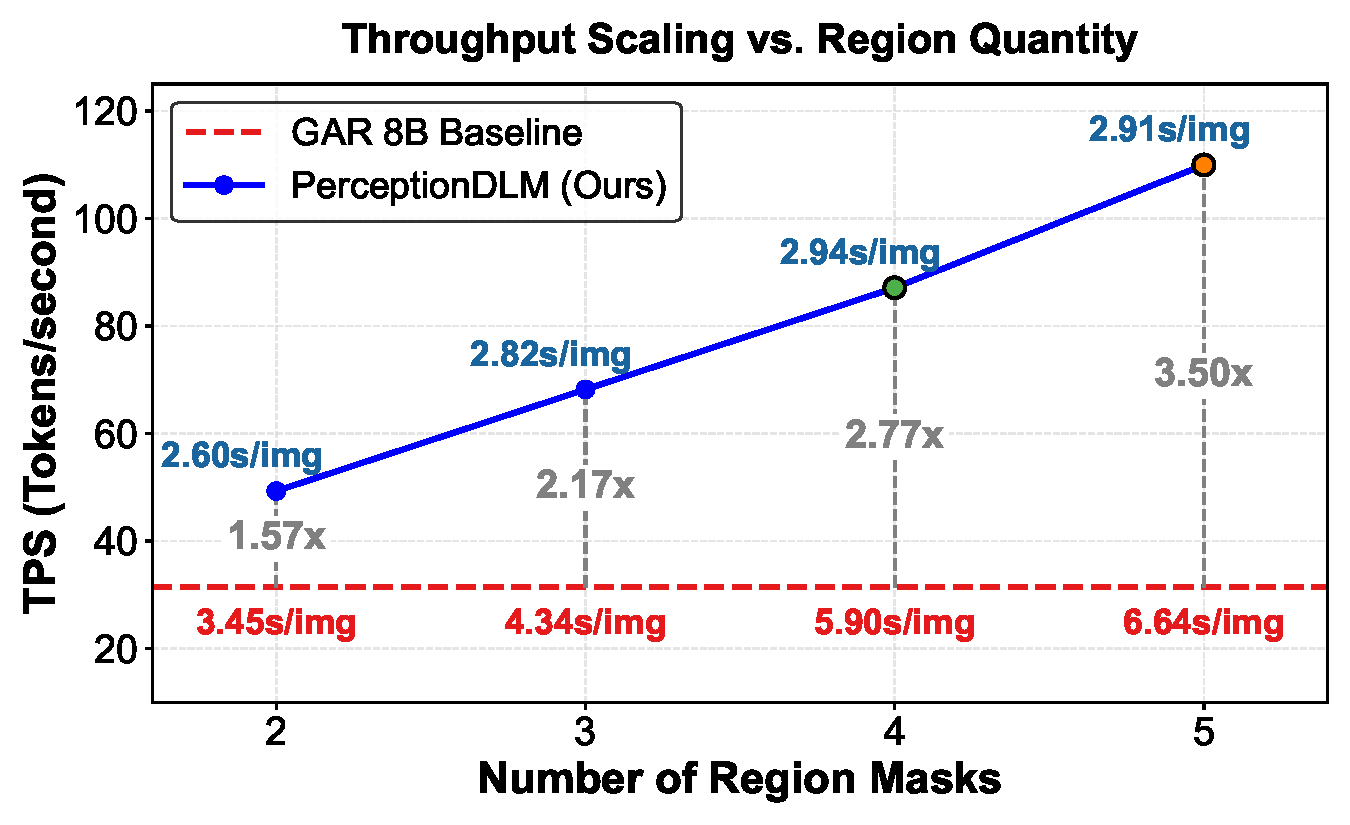
\includegraphics[width=\linewidth]{figs/tps_vs_masks.pdf}
%         \centerline{(a) Throughput vs. Region Quantity}
%     \end{minipage}
%     \hfill % 使用 \hfill 撑开两张图之间的间距
%     \begin{minipage}{0.48\linewidth}
%         \centering
%         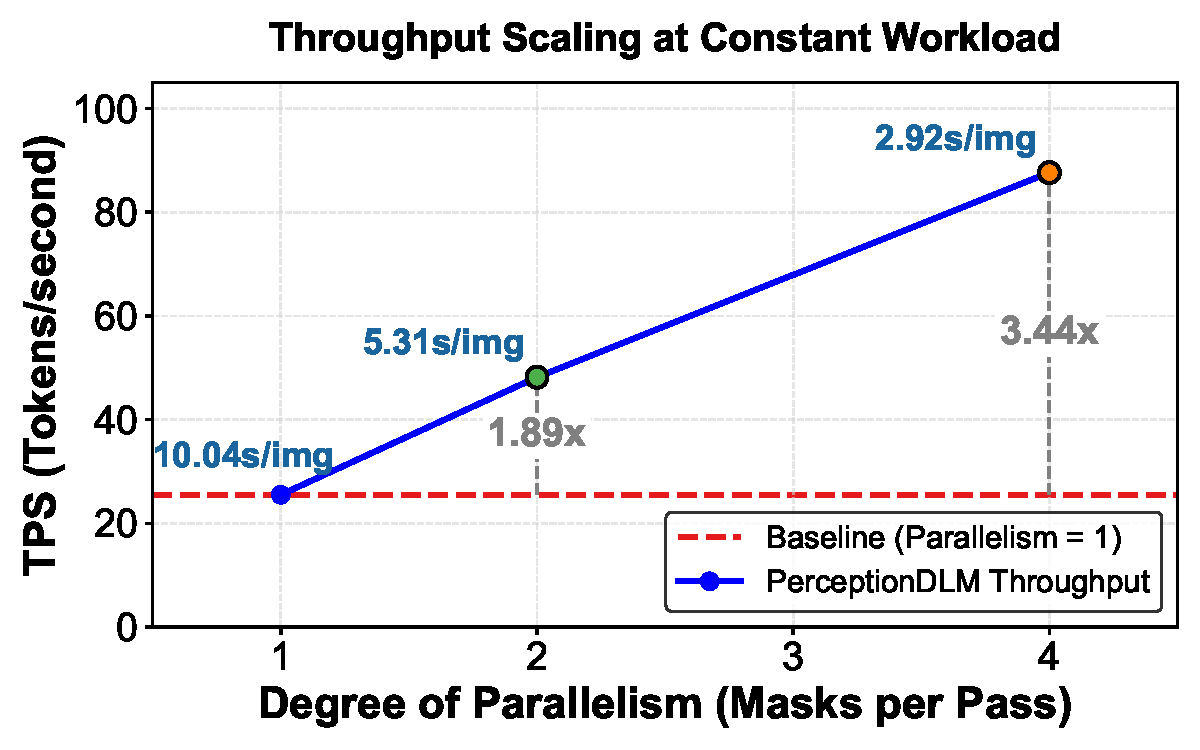
\includegraphics[width=\linewidth]{figs/parallelism_scaling.pdf}
%         \centerline{(b) Throughput Scaling at Constant Workload}
%     \end{minipage}
%     \caption{\textbf{Efficiency and scalability analysis of PerceptionDLM.} 
%     \textbf{(a)} Throughput (TPS) scaling with an increasing number of region masks per image. \textbf{(b)} Parallelism scaling under a constant workload (4 masks per image).}
%     \label{fig:efficiency_analysis}
% \end{figure*}

To systematically analyze the computational advantages of PerceptionDLM, we conduct a speed and efficiency profiling.
% As shown in \Cref{fig:efficiency_analysis}, conventional autoregressive models, such as GAR 8B~\citep{wang2025grasp}, suffer from a sequential bottleneck when processing multiple visual regions, causing per-image latency to scale linearly. In contrast, PerceptionDLM breaks this dependency through non-autoregressive parallel diffusion generation.
As shown in~\Cref{fig:teaser}(b), PerceptionDLM achieves near-linear TPS growth while maintaining stable per-image latency ($\sim$2.9s).
%
In contrast, GAR-8B is bottlenecked at a nearly constant TPS, and its latency degrades approximately linearly with the number of regions. 
%
As shown in~\Cref{fig:teaser}(c), under a constant heavy workload (4 masks per image), increasing the degree of parallelism (masks processed per pass) yields strong scaling for PerceptionDLM: throughput improves by 3.44 times, and single-image latency drops from 10.04s to 2.92s when fully parallelized.